\chapter{音の工学的特徴}
\section{\kadaiaa}\label{sec:\kadaiaa}
\purpose
我々は音の「高い」「低い」をどのようにして認識しているのだろうか.音が高いまたは低いと感じるためには何かと比較するはずだがその比較の指標は何だろうか.
この実験ではまず,正弦波の生成をプログラミングを用いて作成する.そして周波数の変化に対して正弦波グラフおよび音の違いを実験を通して確認し,考察する.
\method
\paragraph{実験に用いる装置}このレポート内全ての実験に用いる言語はMathworks社の\matlab であ理,実行環境は\ref{tbl:実験環境}の通り.
\begin{table}[H]
    \caption{実験環境}
    \label{tbl:実験環境}
    \begin{tabularx}{\textwidth}{AR}
        \hline
        実験機                      & Mac Studio 2022 (Apple社) \\
        プロセッサ                    & Apple Silicon M1 Max     \\
        メモリ                      & 32GB                     \\
        \multirow{2}{*}{\matlab} & R2023a 9.14.02206163     \\
                                 & 64-bit (maci64)          \\
        \hline
    \end{tabularx}
\end{table}
また,このレポートない全ての実験では\matlab でプロットしたグラフを出力するために,関数\ref{src:グラフ出力}を用いている.
\begin{lstlisting}[numbers={none},frame={lines},caption={グラフ出力},label={src:グラフ出力}]
exportgraphics(figurename,'path/figure_name.pdf','ContentType','vecto')
\end{lstlisting}
\paragraph{正弦波について}時刻\(t\)に対して周波数\(f\)の正弦波は,\eqref{equ:正弦波}で得られる.
\begin{align}
    y & =\sin(2\pi ft)\label{equ:正弦波}
\end{align}
時間軸データ\(t\)を\mat{1}{N}のベクトルに代入する.
時間軸データの作成について,サンプリング周波数\texttt{Fs}に対して\(m\)秒間の正弦波を生成するためには,\ref{src:時間軸作成}のように\texttt{0}から\texttt{Fs}まのベクトルに対して,各要素をサンプリング周波数で割ると時間軸テーブルを作成することができる.\par
\begin{wrapfigure}{r}[0mm]{.4\textwidth}
    \begin{lstlisting}[caption={時間軸作成},numbers={none},label={src:時間軸作成}]
t = (0 : m*(Fs-1)) /Fs;
\end{lstlisting}
\end{wrapfigure}
\(t\)の各要素\(t_n\)に対して三角関数\(\sin(2\pi ft_n)\)を演算し,ベクトル\(y\)の要素\(y_n\)に代入する.従って\(y\)も\mat{1}{N}のベクトルになる.
生成した正弦波を\texttt{plot}関数を用いて\(y\)を\(t\)の関数として描画する.このように,ただ一つの正弦波からなるような音を\textbf{純音}という.\cite[p.1]{音響工学理論基礎}
また,サンプリング周波数を\texttt{Fs}とし,データ列\texttt{y}を再生するためには\texttt{sound}関数を用いる.\par
\paragraph{実験内容}この実験では,周波数を\(f_1=440\textrm{Hz}\),\(f_2=660\textrm{Hz}\)の2種類を用いてそれぞれ正弦波\(y_1\),\(y_2\)を生成する.生成した\(y_n(n=\{1,2\})\)に対して,\(t\)を横軸に取りグラフを作成し,サンプリング周波数を\(\textrm{\texttt{Fs}}=16000\textrm{Hz}\)として再生する.\par
\appd{\ref{sec:\kadaiaa}}{src:01_01}
\result
各正弦波のグラフを\ref{fig:\kadaiaa}に示す.音を聴き比べた結果,\(f_2\)の周波数を用いた正弦波は\(f_1\)を用いた正弦波に比べて音が高かった.具体的には\(f_1\)がAの音\footnote{イタリア語音階で「ラ」}であるのに対して,\(f_2\)の音は完全5度大きいEの音\footnote{イタリア語音階で「ミ」}であった.
\begin{wrapfigure}{r}[0mm]{.3\textwidth}
    \caption{周波数が異なる正弦波のグラフ}
    \label{fig:\kadaiaa}
    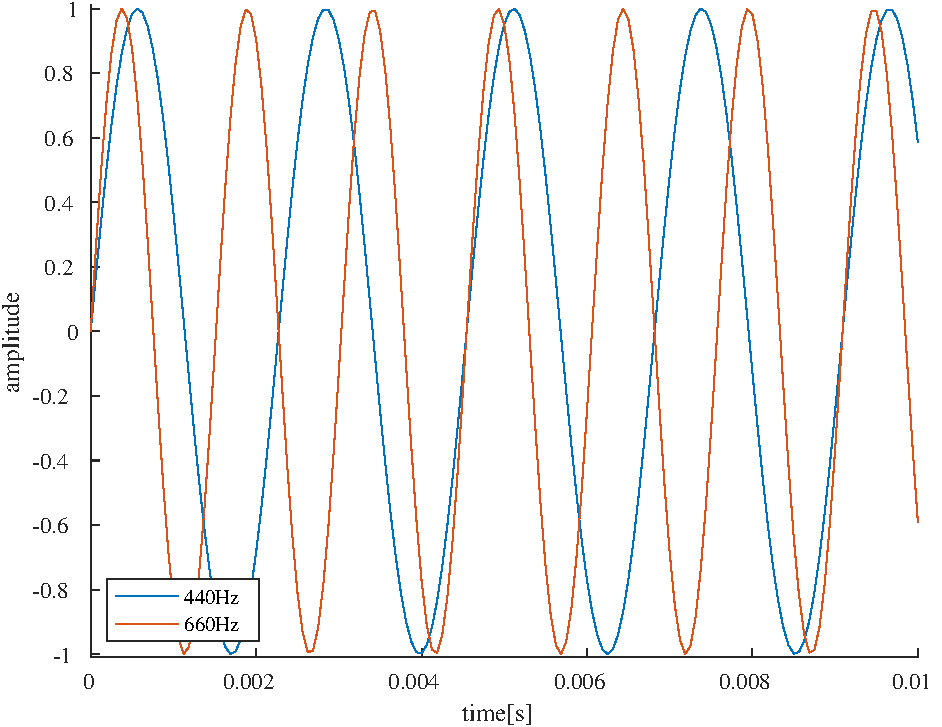
\includegraphics[keepaspectratio,width=.3\textwidth]{../../Figures/01_01.pdf}
\end{wrapfigure}
さらに,聴音確認・目視確認では音の大きさ,音色,振幅や波形の変化は確認でなかった.\par
\consideration 周波数\ \((f)\)\ とは1秒間の振動回数であり,これが音の高さを決める.実験結果より周波数が大きい,つまり1秒間により多く振動すれば音が高くなることが分かった.
また,1回振動あたりの時間を周期\ \((T)\)\ と言うが,周期と周波数は反比例の関係であり,\eqref{equ:周期と周波数}が成り立つ.
\begin{align}
    f & =\frac{1}{T} & \big(\textrm{無論}\quad T\neq 0,\quad f\neq 0\big)\label{equ:周期と周波数}
\end{align}
\ref{fig:周波数の異なる純音の生成}より,周波数が大きい正弦波は周期が短く,逆もまた確認できる.
周波数のみを変更したので,振幅や正弦波の波形変化はない.\par
また,周波数が\(f_1\)正弦波の音と\(f_2\)正弦波の音はそれぞれ純音だがこれらの間にも関係がある.数学的には\(f_1:f_2=2:3\)の簡単な整数比になっている.
\begin{leftbar}
    ヒトの耳は2つの音を同時に聞いた場合,その2つの音の周波数が簡単になっているほど協和して聴こえる.(略)\par
    このように周波数比が整数比になっている音程を純音程とよぶ.\hfill{\cite[p.46-p.47]{音響工学理論基礎}}
\end{leftbar}
つまり,周波数\(f_1\)正弦波と周波数\(f_2\)正弦波の加算合成波はは協和してきこえる.
\section{\kadaiab}\label{sec:\kadaiab}
\purpose
音の大小は何によって決まるのだろうか.音の大小に関わる波の振幅や,波を構成する上で重要な初期位相を変化させ,変化の前後での音の違いを聞き取り,人間の耳に初期位相の変化や振幅の変化がどのように感じるか実験を通して考察する.
\method
時刻\(t\)に対して周波数\(f\)の正弦波は\eqref{equ:正弦波}で得られるが,その初期位相(\textit{initial phase})を\(\phi\)とすると,その正弦波は\eqref{equ:正弦波_初期位相}となる.
\begin{align}
    y & =\sin(2\pi ft+\phi)\label{equ:正弦波_初期位相}
\end{align}また,同様な正弦波:\eqref{equ:正弦波}の振幅を\(A\)倍して得られる正弦波は\eqref{equ:正弦波_振幅}となる.
\begin{align}
    y & =A\sin(2\pi ft)\label{equ:正弦波_振幅}
\end{align}
\paragraph{実験内容}この実験では,初期位相の変化と振幅の変化,それぞれ実験し変化前と変化後の音や波形の違いを発見する.周波数は\(f=440\textrm{Hz}\)とし,サンプリング周波数を\(\texttt{Fs}=16000\textrm{Hz}\)とする.
左から純音,右から波長や初期位相を変化させた音を再生するようにして(\ref{src:左右から別の音を出力}),音の変化を確認する.\appd{\ref{sec:\kadaiab}}{src:01_02}
\begin{lstlisting}[caption={左右から別の音を出力},label={src:左右から別の音を出力},numbers={none}]
Fs = 16000; % サンプリング周波数
y1 = 音声データ1; % N行1列(左)
y2 = 音声データ2; % N行1列(右)
y = [y1 y2]; % N行2列 列結合を行う
sound(y, Fs); 
\end{lstlisting}
\begin{table}[h]
    \caption{\kadaiab\ 実験内容}
    \label{tbl:\kadaiab_実験内容}
    \begin{tabularx}{\textwidth}{RCCR}
        \multicolumn{1}{c}{\textbf{実験対象}} & \multicolumn{1}{c}{\textbf{振幅(基準倍)}} & \multicolumn{1}{c}{\textbf{初期位相}} & \multicolumn{1}{c}{\textbf{生成される正弦波}} \\
        \hline
        純音                                & 基準                                   & 基準                                & \(y_0=\sin(2\pi ft)\)                 \\
        \hline
        \multirow{2}{*}{振幅}               & \(0.5\)                              & \(0\)                             & \(y_1=0.5\times\sin(2\pi ft)\)        \\
                                          & \(0.25\)                             & \(0\)                             & \(y_2=0.25\times\sin(2\pi ft)\)       \\
        \hline
        \multirow{2}{*}{初期位相}             & \(1\)                                & \(+\frac{\pi}{2}\)                & \(y_3=\sin(2\pi ft+\frac{\pi}{2})\)   \\
                                          & \(1\)                                & \(+\pi\)                          & \(y_4=\sin(2\pi ft+\pi)\)             \\
        \hline
    \end{tabularx}
\end{table}
\result
聴音確認の結果を\ref{tbl:\kadaiab_実験結果},\ref{fig:振幅・位相の確認_結果_振幅}及び\ref{fig:振幅・位相の確認_結果_初期位相}に示す.振幅の変化について,振幅の変化に比例した音量変化を確認できたが,初期位相の変化による音の変化は確認できなかった.
\begin{table}[H]
    \caption{\kadaiab\ 実験結果}
    \label{tbl:\kadaiab_実験結果}
    \begin{tabularx}{\textwidth}{ccclR}
        \multicolumn{1}{c}{\textbf{実験対象}} & \multicolumn{1}{c}{\textbf{振幅(基準倍)}} & \multicolumn{1}{c}{\textbf{初期位相}} & \multicolumn{1}{c}{\textbf{生成される正弦波}} & \multicolumn{1}{c}{\textbf{純音との比較}} \\
        \hline
        純音                                & 基準                                   & 基準                                & \(y_0=\sin(2\pi ft)\)                 & \multicolumn{1}{c}{ー}               \\
        \hline
        \multirow{2}{*}{振幅}               & \(0.5\)                              & \(0\)                             & \(y_1=0.5\times\sin(2\pi ft)\)        & 音量がおおよそ\(1/2\)に聞こえた.                \\
                                          & \(0.25\)                             & \(0\)                             & \(y_2=0.25\times\sin(2\pi ft)\)       & 音量がおおよそ\(1/4\)に聞こえた.                \\
        \hline
        \multirow{2}{*}{初期位相}             & \(1\)                                & \(+\frac{\pi}{2}\)                & \(y_3=\sin(2\pi ft+\frac{\pi}{2})\)   & 違いは分からなかった.                         \\
                                          & \(1\)                                & \(+\pi\)                          & \(y_4=\sin(2\pi ft+\pi)\)             & 違いは分からなかった.                         \\
        \hline
    \end{tabularx}
\end{table}
\begin{figure}[H]
    \centering
    \begin{minipage}[t]{.48\textwidth}
        \centering
        \caption{\kadaiab\ 実験結果(振幅の変化)}
        \label{fig:\kadaiab_結果_振幅}
        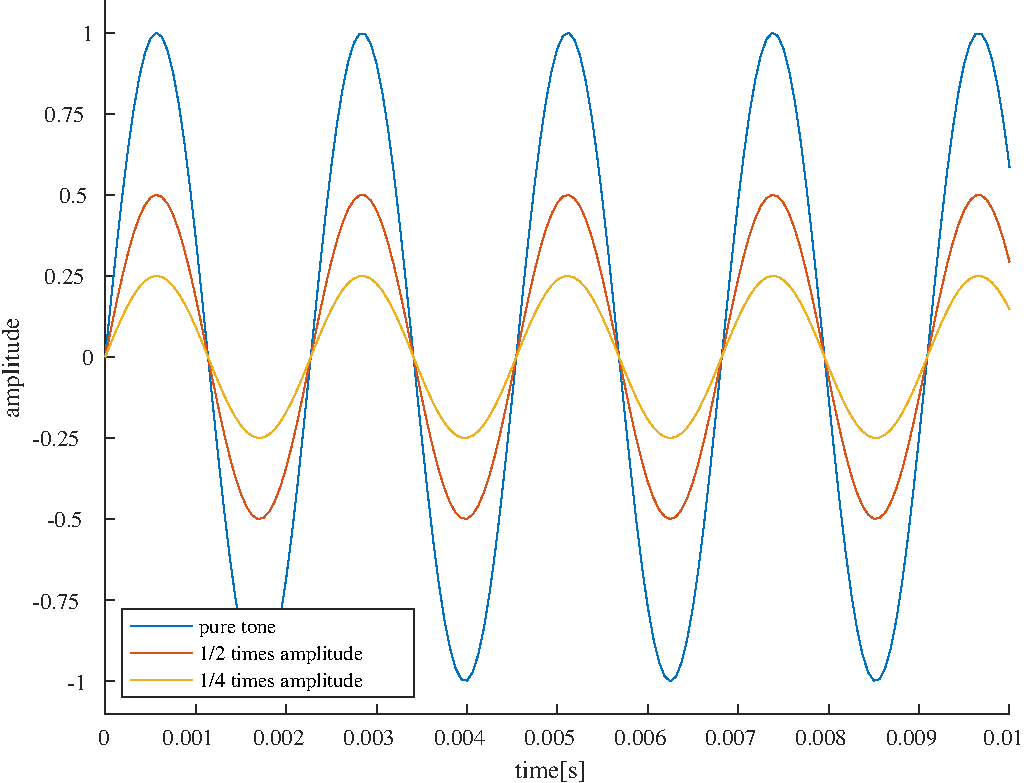
\includegraphics[keepaspectratio,width=\textwidth]{../../Figures/01_02_1.pdf}
    \end{minipage}
    \begin{minipage}[t]{.48\textwidth}
        \centering
        \caption{\kadaiab\ 実験結果(初期位相の変化)}
        \label{fig:\kadaiab_結果_初期位相}
        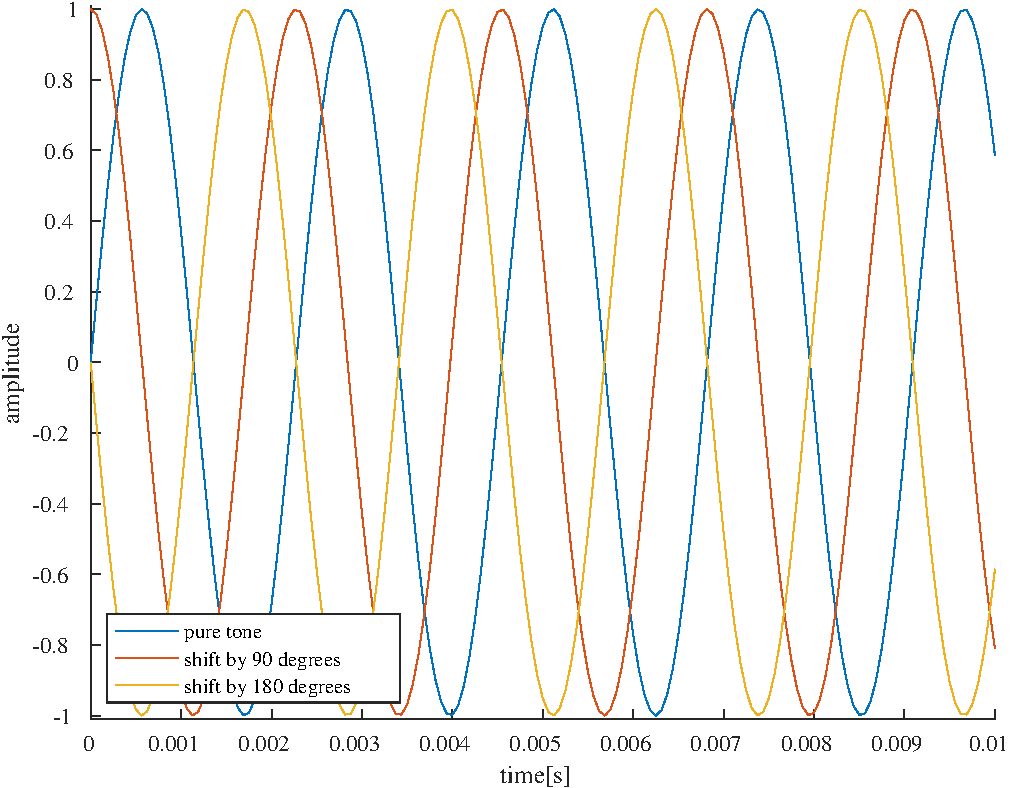
\includegraphics[keepaspectratio,width=\textwidth]{../../Figures/01_02_2.pdf}
    \end{minipage}
\end{figure}
\consideration
\paragraph{振幅の変化について} 振幅の変化は,音量と比例することを確認できた.\ref{fig:振幅・位相の確認_結果_振幅}より,各正弦波において周期や初期位相が等しいので,縦軸が\(0\)になる時刻や最大値を迎えるは等しいく,振幅のみが異なる.
\paragraph{初期位相の変化について} 位相の変化による音の変化は確認できなかった.\ref{fig:振幅・位相の確認_結果_初期位相}より,振幅や周期は等しいが,初期位相が異なるため最小値や最大値を迎える時刻が初期位相分異なる.
\section{\kadaiac}\label{sec:\kadaiac}
\purpose
ティンパニやギターのチューニングを行うとき,音叉やチューナーから音を出して,異なる互いに周波数であれば気づきチューニングする.それぞれ異なる周波数が異なる周波数が周波数の違いによるうなりの発生やその原因を数学的観点から考察する.
\method
うなりとは,異なる周波数が干渉するとき起こる現象である.異なる周波数同士の正弦波が干渉することで,強め合いの場所と弱め合いの場所が周期的に現れることで発生する.
例えば周波数\(f_1\)の正弦波に対して周波数\(f_2(\neq f_1)\)の正弦波を干渉させると,\eqref{equ:うなり}より\(1\)秒間に\(N\)回のうなりを聞くことができる.
\begin{align}
    N & = \big|f_1-f_2\big|\label{equ:うなり}
\end{align}
\(f_1\)と\(f_2\)の差が大きければ,当然うなり(\(N\))の回数は多くなり,\(f_1\)と\(f_2\)の差が小さければうなりの回数は少なくなる.\par
本実験では,サンプリング周波数を\(\texttt{Fs}=16000\textrm{Hz}\),提示時間\(4\)秒,周波数が\(f_1=440\textrm{Hz}\),\(f_2=441\textrm{Hz}\)の純音を加算合成した波形を生成し再生する.\appd{\ref{sec:\kadaiac}}{src:01_03}\par
\begin{wrapfigure}{r}[0mm]{.3\textwidth}
    \centering
    \caption{\kadaiac\ 実験結果}
    \label{fig:\kadaiac_実験結果}
    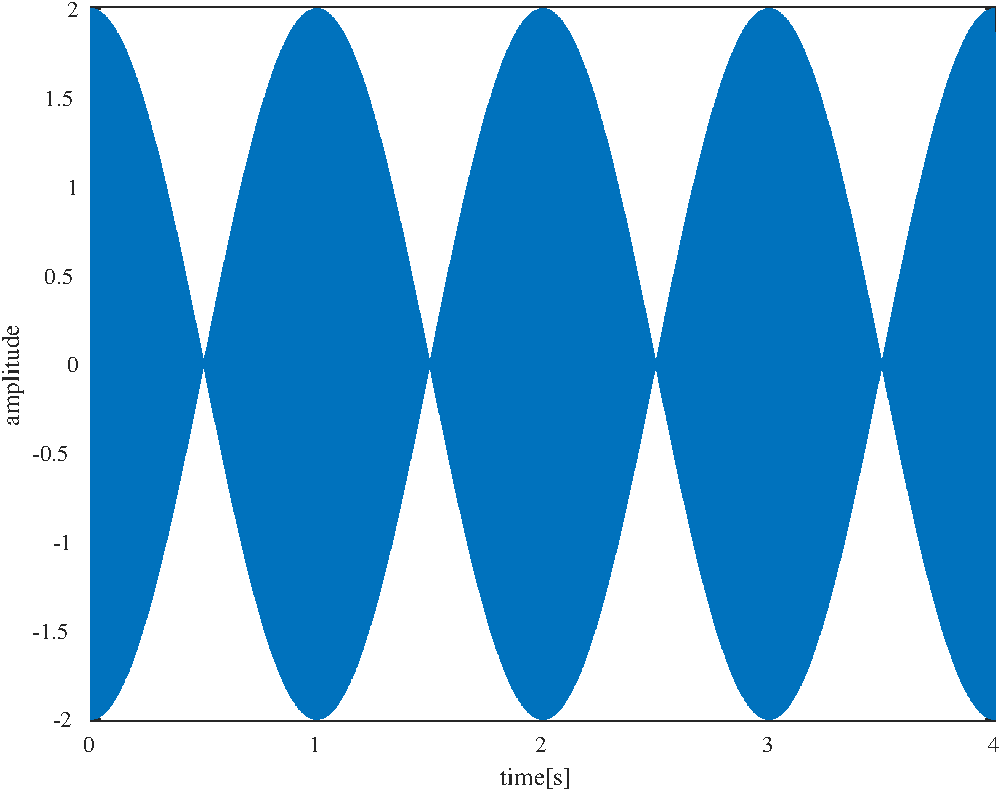
\includegraphics[keepaspectratio,width=.3\textwidth]{../../Figures/01_03.pdf}
\end{wrapfigure}
\result
うなりは4回聞こえた.また,時間軸に対して加算合成したデータを描画すると\ref{fig:\kadaiac_実験結果}となった.
\consideration \eqref{equ:うなり}に従って,
\begin{equation}
    \begin{aligned}
        \big|f_1-f_2\big| & = \big|440-441\big| \\
                          & =1
    \end{aligned}
\end{equation}
より\(1\)秒あたり\(1\)回のうなりが聞こえるはずなので,この実験結果は論理的に正しい.
加算合成波\ref{fig:\kadaiac_実験結果}の振幅に着目しても,周波数\(f_1\),\(f_2\)それぞれの正弦波の振幅が1であることを考えると,その加算合成波の振幅が2であることも理解できる.
さらに,この加算合成波は\(t=0\)のとき最大値を迎えており,これは初期位相が同一の正弦波の加算合成であることを表している.
\section{\kadaiad}
\purpose
矩形波は周期関数だが,見た目は正弦波ではない.これをプログラム上でどのように再現するのか.フーリエ級数展開を用いた矩形波の描画やフーリエ級数展開のプログラム上で再現し,理想的な矩形波との比較を行う.
\method
\paragraph{フーリエ級数展開}周期\(T\)の任意の周期信号\(f(t)\)に対して,それはより短い周期\(T/n(n=1,2,\dots)\)を持つ正弦波の重ね合わせで表すことができる.具体的には\eqref{equ:フーリエ級数展開}で表すことができ,これをフーリエ級数展開という.\cite[p.18-p.19]{信号処理}
\begin{align}
    f(t) & =\frac{1}{2}a_0 + \sum_{k=1}^{\infty}\big(a_k\cos(k\omega_0t)+b_k\sin(k\omega_0t)\big) & \omega_0 & =\frac{2\pi}{T}\label{equ:フーリエ級数展開}  \\
    f(t) & =\frac{1}{2}a_0 + \sum_{k=1}^{N}\big(a_k\cos(k\omega_0t)+b_k\sin(k\omega_0t)\big)      & \omega_0 & =\frac{2\pi}{T}\label{equ:フーリエ級数展開N}
\end{align}
特に\eqref{equ:フーリエ級数展開N}の\(N=1\)の時を基本周波数と呼ぶ.\\
\begin{wrapfigure}{r}[0mm]{.3\textwidth}
    \caption{矩形波(\(1\leq k\leq 50\))}
    \label{fig:矩形波}
    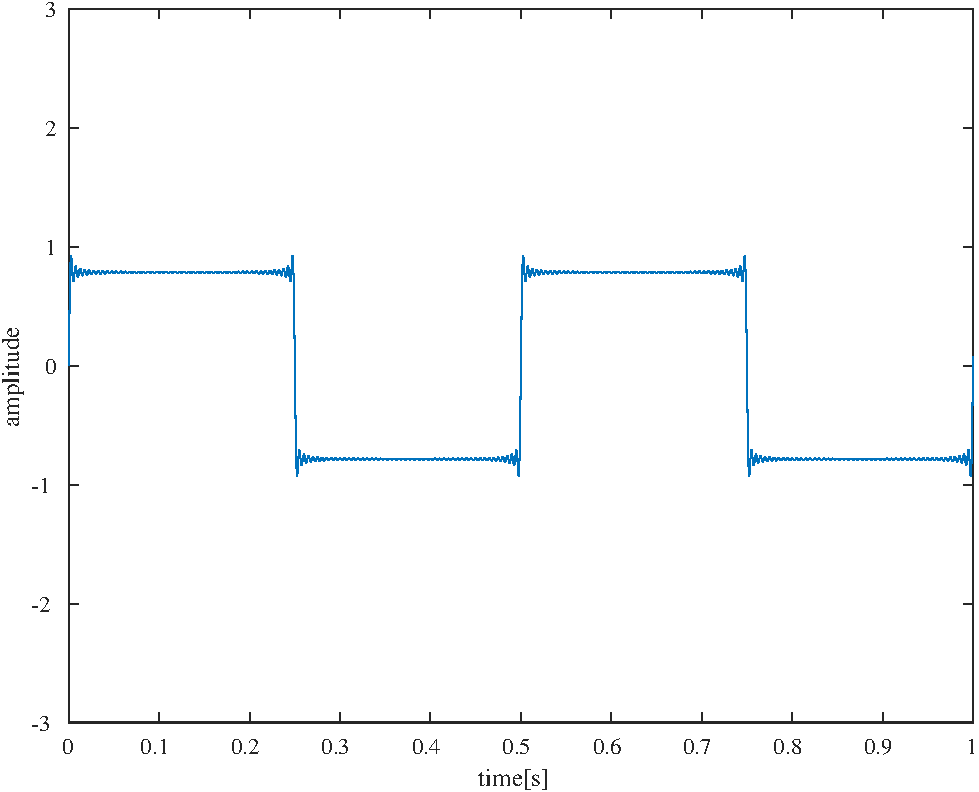
\includegraphics[keepaspectratio,width=.3\textwidth]{../../Figures/01_04_1.pdf}
\end{wrapfigure}
\paragraph{矩形波}
矩形波は周期関数である.その周期を\(T\)とすると,関数\(f\)は時刻\(t\)に対して,フーリエ級数展開するとになる.\eqref{equ:矩形波}は周期\(T=1/2\)で定義した矩形波で,\eqref{equ:矩形波N}を\(N=50\)で出力した.\par
\begin{align}
    f(t) & =\sum_{k=1}^{\infty}\frac{1}{2k-1}\sin\big(2\pi(2k-1)ft\big)\label{equ:矩形波} \\
    f(t) & =\sum_{k=1}^{N}\frac{1}{2k-1}\sin\big(2\pi(2k-1)ft\big)\label{equ:矩形波N}
\end{align}
\paragraph{実験内容}周期\(T=1/2\)として,\eqref{equ:矩形波N}の\(N\)の値を\(N=1, 5, 25\)と増やした時に次第に波形が矩形波に収束していくことを確認する.
\result
\begin{wrapfigure}{r}[0mm]{.3\textwidth}
    \centering
    \caption{\kadaiad\ 実験結果}
    \label{fig:\kadaiae_実験結果}
    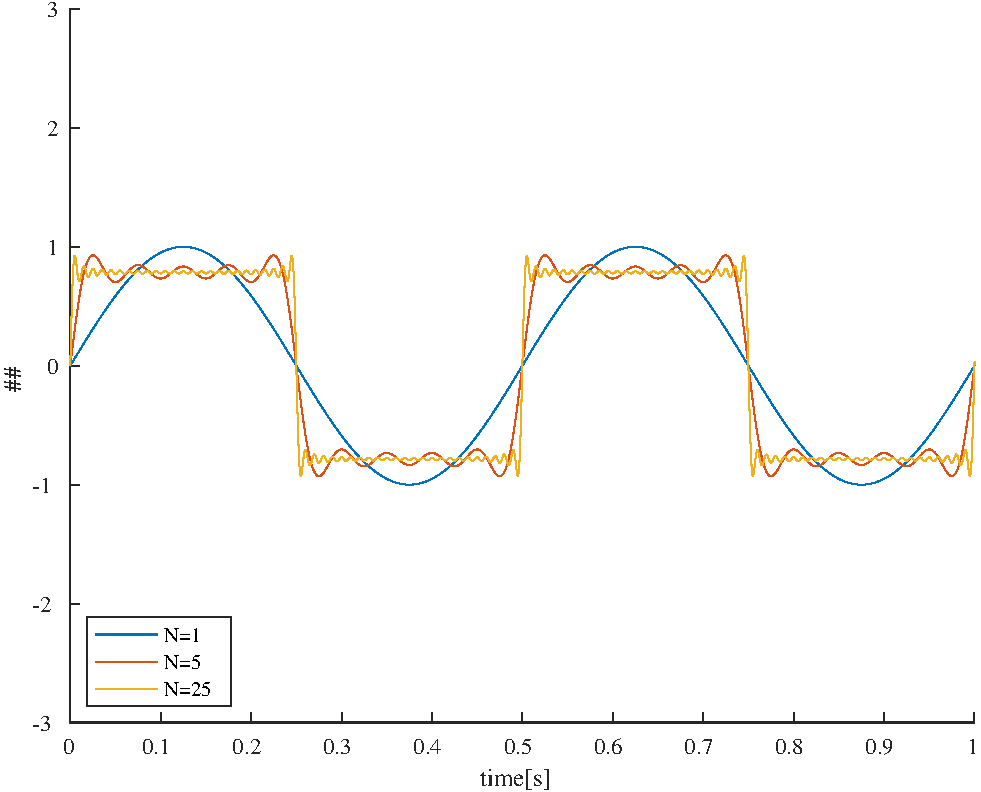
\includegraphics[keepaspectratio,width=.3\textwidth]{../../Figures/01_04_2.pdf}
\end{wrapfigure}
\ref{fig:\kadaiae_実験結果}の通り,\(N\)を大きくすると,矩形波に収束することがわかった.また,基本周波数と矩形波の周期も目測では一致している.
\consideration
計算機を用いて\(N\)の値を無限大で出力することは不可能である.\ref{fig:矩形波}のように\(N=50\)として出力すると,理想的な矩形波に近づくが完全ではない.ここで\(N\)の値を大きくすると,周期
\section{\kadaiae}
\purpose